\documentclass[10pt,twocolumn,letterpaper]{article}

%==================== PACCHETTI ====================
\usepackage[T1]{fontenc}
\usepackage[utf8]{inputenc}
\usepackage{times}
\usepackage[margin=0.75in,columnsep=0.25in]{geometry}
\usepackage{graphicx}
\usepackage{amsmath,amssymb}
\usepackage{booktabs}
\usepackage{enumitem}
\usepackage{hyperref}
\usepackage{xcolor}
\usepackage{caption}
\usepackage{subcaption}
\usepackage{listings}
\usepackage{titlesec}
\usepackage{fancyhdr}
\usepackage{framed}

\hypersetup{colorlinks=true,linkcolor=black,citecolor=black,urlcolor=blue}

%==================== STILE SEZIONI (stile CVPR) ====================
\titleformat{\section}{\normalfont\large\bfseries}{\thesection.}{0.6em}{}
\titleformat{\subsection}{\normalfont\normalsize\bfseries}{\thesubsection.}{0.6em}{}
\titleformat{\subsubsection}{\normalfont\normalsize\bfseries\itshape}{\thesubsubsection}{0.6em}{}
\titlespacing*{\section}{0pt}{2.2ex plus 1ex minus .2ex}{1.3ex plus .2ex}
\titlespacing*{\subsection}{0pt}{2.0ex plus 1ex minus .2ex}{1.0ex plus .2ex}

\setlength{\parindent}{1em}
\setlength{\parskip}{0pt}

\pagestyle{plain}

%==================== CODICE ====================
\lstset{
  basicstyle=\ttfamily\footnotesize,
  columns=fullflexible,
  breaklines=true,
  frame=single,
  backgroundcolor=\color{gray!8},
  xleftmargin=0.5em,
  xrightmargin=0.5em,
}

%==================== TITOLO / ABSTRACT (stile CVPR: full-width prima delle due colonne) ====================
\newcommand{\reporttitle}{Parallel Programming for Computer Graphics\\[2pt]
\large Mid-term project: \textit{2D Circle Rasterization}}

\begin{document}

\twocolumn[
  {\centering
   {\LARGE \bfseries Parallel Programming for Computer Graphics \\[4pt]}
   {\Large Mid-term project: \textit{2D Circle Rasterization} \\[10pt]}
   {\large Francesco Acciaioli \\}
   {University of Florence \\}
   {\ttfamily\small francesco.acciaioli@stud.unifi.it \\[10pt]}
  }

  \vspace{6pt}
]

%==================== ABSTRACT (mezza colonna) ====================
\begin{center}\large\textbf{Abstract}\end{center}
\vspace{-4pt}
\begin{list}{}{\setlength{\leftmargin}{1.5em}\setlength{\rightmargin}{1.5em}}\item[]
\small\itshape
  Rasterizing large numbers of alpha-blended, depth-ordered 2D primitives is a core building
  block of real-time and offline rendering, and it is embarrassingly parallel in principle but
  easy to implement inefficiently. This report presents a CPU-only 2D circle rasterizer,
  implemented in Python with Numba, that draws $N$ alpha-blended circles onto an $H\times W$
  image using the painter's algorithm. Four kernels of increasing sophistication are compared:
  a sequential baseline, a naive per-pixel parallel kernel, a tile-based parallel kernel with
  bounding-box culling, and a tile-based kernel additionally written for auto-vectorization
  (branchless SIMD inner loop). On an 8-core Apple Silicon (M2) machine, the tiled, vectorized
  kernel reaches a maximum speedup of \textbf{9.1$\times$} over the sequential baseline (on
  16 oversubscribed threads), while a dedicated scalar-vs-SIMD comparison shows vectorization
  alone contributes roughly \textbf{4$\times$} (3.6--5.5$\times$) at a fixed thread count. A broader set of
  micro-benchmarks additionally isolates the effect of resolution, circle count, tile size,
  memory layout (SoA vs.\ AoS) and weak scaling, providing a systematic picture of where the
  performance comes from and where it saturates.
  \end{list}

\vspace{4pt}
\noindent{\large\textbf{Future Distribution Permission}}\\
The author(s) of this report give permission for this document to be distributed to
Unifi-affiliated students taking future courses.


%==================================================================
\section{Introduction}

This report presents the design, implementation and performance analysis of a
sequential and parallelized 2D circle rasterizer. The project was developed for
the \emph{Parallel Programming} course to demonstrate how coarse-grained
multithreading and fine-grained vectorization can be combined to accelerate a
classic, embarrassingly-parallel computer-graphics workload.

\subsection{Problem Description and Motivation}

Rasterization is the process of converting geometric primitives into pixels.
This project targets a deliberately simple but representative primitive set:
$N$ circles, each defined by a 2D center, a depth coordinate $z$, a radius, an
RGB color and an alpha (opacity) value. Circles are composited onto the image
using the \emph{painter's algorithm}: they are sorted by increasing depth and
drawn back-to-front, blending each new circle onto the frame buffer with the
standard ``over'' operator
\[
  \text{out} = \text{src}_{\text{rgb}}\cdot a + \text{dst}_{\text{rgb}} \cdot (1-a).
\]
This is the same compositing model used by real rendering pipelines (e.g.\
particle systems, 2D vector graphics, UI compositors), which makes the problem
a realistic, minimal stand-in for a much larger class of rendering workloads.

\subsection{Computational Challenges}

A pixel $(i,j)$ belongs to circle $k$ if its center $(i+0.5,\,j+0.5)$ satisfies
$dx^2+dy^2 \le r_k^2$. In the naive formulation every one of the $H\times W$
pixels must be tested against every one of the $N$ circles, giving
$O(H\cdot W\cdot N)$ work per frame. Even after restricting each circle to its
axis-aligned bounding box, the workload remains large and highly
\emph{irregular}: circles vary enormously in radius (a few pixels up to
$\sim\!12\%$ of the image side), so the amount of work associated with
different pixels — and with different spatial tiles of the image — is far
from uniform. This irregularity, rather than raw arithmetic volume, is the
central challenge that the parallelization strategy has to address.

\subsection{Objectives and Scope}

The goal of the project is to explore, in a controlled way, which parallelization
and vectorization techniques are effective for this class of workload, and why.
The scope includes:
\begin{enumerate}[itemsep=1pt,topsep=2pt]
  \item \textbf{Sequential implementation:} a straightforward, single-threaded
    kernel used as the correctness and performance baseline.
  \item \textbf{Parallel optimization:} two coarse-grained multithreaded
    strategies (per-pixel-row and per-tile), plus a tile-based kernel whose
    inner loop is written to be auto-vectorized by the compiler.
  \item \textbf{Systematic micro-benchmarking:} isolating, one variable at a
    time, the effect of thread count, image resolution, circle count, tile
    size, SIMD, memory layout and weak scaling.
\end{enumerate}

%==================================================================
\section{Algorithm Description}

\subsection{Data Structure}

Circles are stored in a \emph{Structure-of-Arrays} (SoA) container
(\texttt{CircleSoA}): eight parallel, contiguous \texttt{float32} NumPy arrays
$(x, y, z, \text{radius}, r, g, b, a)$, rather than a list of per-circle
objects. This layout is cache-friendly and is the natural starting point for
vectorization, since each attribute is unit-stride in memory~\cite{robey}. Sorting by depth
is done once, up front, with a \emph{stable} mergesort, so that circles with
equal $z$ keep their original (insertion) order deterministically; the sort
is never repeated inside a rendering kernel.

\subsection{Sequential Algorithm}

The baseline kernel loops over circles from far to near. For each circle it
computes an integer bounding box clipped to the image, then scans only the
pixels inside that box, testing the circle equation and applying the ``over''
blend in place:

\begin{lstlisting}
for k in range(n):            # far -> near
    x0,y0,x1,y1 = bbox(k)     # clipped to image
    for j in range(y0, y1):
        for i in range(x0, x1):
            if inside_circle(i, j, k):
                blend_over(img[j, i], color(k))
\end{lstlisting}

This bounding-box restriction is the only optimization present in the
sequential version; it is still $O(N)$ circles times, on average,
$O(r_k^2)$ pixels, and it writes directly into a shared image buffer, which
is safe here only because the loop is single-threaded.

\subsection{Parallelization Strategy}

Two independent opportunities for parallelism were identified:

\paragraph{Parallelizing across the image (multithreading).} Because the
final color of a pixel does not depend on the color of any other pixel
(circles are looked up, not accumulated across pixels), the image can be
partitioned into disjoint regions — rows or square tiles — and each region
processed independently by a different thread, with no shared mutable state
and therefore no locks.

\paragraph{Vectorizing the inner loop (SIMD).} Inside a tile, testing a
circle against many pixels performs the same arithmetic (subtraction,
multiplication, comparison, blend) on independent data. If that inner loop is
written without early-exit branches and with a small, contiguous, per-tile
buffer, the compiler's auto-vectorizer can turn it into SIMD instructions
that process several pixels per cycle.

%==================================================================
\section{Parallel Implementation}

Four rendering kernels are implemented and compiled just-in-time with Numba, which
generates native code through LLVM
(\texttt{@njit}); they are referred to as \texttt{seq},
\texttt{pixels}, \texttt{tiles} and \texttt{simd}, and all four are required to
produce the same image (up to floating-point reassociation error from
\texttt{fastmath}).

\subsection{Strategy Overview}

\begin{table}[h]
\centering
\small
\begin{tabular}{@{}lll@{}}
\toprule
\textbf{Mode} & \textbf{Parallelism} & \textbf{Notes} \\
\midrule
\texttt{seq}    & none              & baseline, bbox scan \\
\texttt{pixels} & \texttt{prange} over rows   & no culling, slow \\
\texttt{tiles}  & \texttt{prange} over tiles  & bbox culling per tile \\
\texttt{simd}   & tiles + vector inner loop & fastest, branchless \\
\bottomrule
\end{tabular}
\caption{The four rendering kernels compared in this project.}
\label{tab:kernels}
\end{table}

\texttt{pixels} parallelizes Numba's \texttt{prange} over image rows: each
thread owns a disjoint set of rows and, for every pixel, loops over \emph{all}
$N$ circles with a cheap bounding-box rejection test. It has no spatial
culling structure, so it is included mainly as a ``multithreading alone''
reference point — it is intentionally slow.

\texttt{tiles} instead parallelizes over square tiles of the image. For each
tile, a thread-local candidate list is built once by testing which circles'
bounding boxes intersect the tile; only that (usually much smaller) candidate
set is then scanned against every pixel of the tile. Disjoint tiles mean
disjoint writes, so again no synchronization is needed.

\texttt{simd} uses the same tile/culling structure as \texttt{tiles}, but the
inner double loop over a tile's pixels is restructured for auto-vectorization:
for each candidate circle, all pixels of the tile are visited in a countable,
branch-free loop that computes a $0/1$ mask instead of using an \texttt{if},
and pixels are accumulated into small contiguous per-tile R/G/B scratch
buffers before being written back to the image once at the end:

\begin{lstlisting}
for ii in range(tw):                # vectorizable
    d2 = dx*dx + dy2                # FMA under fastmath
    m = 1.0 if d2 <= r2 else 0.0    # branchless mask
    rr[idx] = m*(psr + rr[idx]*inv) + (1-m)*rr[idx]
\end{lstlisting}

Removing the branch and keeping the accumulator arrays contiguous and small
(tile-sized) lets LLVM auto-vectorize the loop with unit-stride vector
loads/stores, and lets \texttt{fastmath=True} fuse the distance computation
into fused multiply-adds.

\subsection{Load Balancing: prange and Scheduling}

Numba's \texttt{prange} is the direct analogue of an OpenMP
\texttt{\#pragma omp parallel for}: it distributes loop iterations (rows, or
tiles) across the threads set by \texttt{numba.set\_num\_threads()}. Because
circle radii vary widely, the amount of work per tile is highly non-uniform
(a tile with only small, sparse circles finishes almost instantly; a tile
covered by several large overlapping circles is far more expensive). This is
exactly the kind of irregular workload for which \emph{dynamic} scheduling is
preferable to static partitioning. Unlike OpenMP, however, \texttt{prange}
has no \texttt{schedule(static|dynamic|guided)} clause, so the three
strategies cannot be compared directly. By default Numba splits the iteration
space into roughly equal contiguous blocks, one per thread, which behaves like
\texttt{schedule(static)}. The load is balanced instead by
splitting the image into many small tiles (many more tiles than threads):
each thread's block then contains many tiles, so cheap and expensive tiles
average out. This is why the tile size is studied explicitly in
Section~\ref{sec:results}.

\subsection{Synchronization}

By construction, every kernel here operates on disjoint output regions
(rows or tiles), so the renderer itself is \textbf{lock-free}: no shared
mutable accumulator is ever written by more than one thread, and no locks,
atomics or critical sections are required.

\subsection{Data Structures and Memory Layout}

The default layout is SoA, as described above. For comparison, a
\texttt{to\_aos()} conversion produces an interleaved $(N,8)$
\emph{Array-of-Structures} layout, used only by the memory-layout benchmark
(Section~\ref{sec:memlayout}); the renderer itself never uses it internally.

%==================================================================
\section{Experimental Setup}

\subsection{Environment}

Benchmarks were executed on an Apple Silicon MacBook Air \textbf{M2 (ARM64)}, a
hybrid design with 4 performance and 4 efficiency cores (8 logical/physical
cores reported by the OS). The software stack was Python 3.11.9, NumPy 2.4.6,
Numba 0.67.0 and llvmlite 0.49.0 on macOS. Numba's thread ceiling
(\texttt{NUMBA\_NUM\_THREADS}) was deliberately set to \textbf{16}, i.e.\
\emph{twice} the number of logical cores, so that the thread-scaling
experiment can observe oversubscription behavior (thread count exceeding the
physical core count) as required by the course guidelines~\cite{slides}, in addition to
normal scaling up to the core count. The MacBook Air is fanless, so under
sustained all-core load it reduces its clock frequency (thermal throttling):
single-threaded timings were reproducible across runs, while multi-threaded
timings varied by up to $\sim\!20\%$ between runs. Multi-threaded results
should therefore be read as trends rather than exact values.

\subsection{Dataset}

The dataset is procedurally generated: $N$ circles with uniformly random
position, radius (scaled to image resolution), color and alpha. This is a
deliberate choice rather than a limitation — for a 2D rasterizer,
synthetically generated geometry \emph{is} the realistic workload, in the
same way standard rasterization benchmarks use synthetic scenes rather than
an external image dataset; there is no natural pre-existing dataset of
``circles with depth and alpha'' to substitute.

\subsection{Methodology and Parameters}

\begin{itemize}[itemsep=1pt,topsep=2pt]
  \item \textbf{Timing:} wall-clock time via \texttt{time.perf\_counter}
    equivalents, with a per-configuration time budget that stops adding
    iterations once exceeded (bounding the cost of slow configurations), plus
    CPU time (\texttt{time.process\_time()}, summed across threads) and an
    approximate 95\% confidence interval ($1.96\cdot\sigma/\sqrt{n}$).
  \item \textbf{Warm-up:} each configuration is preceded by 2 warm-up runs
    (excluded from timing) to absorb Numba's JIT compilation cost; kernels are
    also cached to disk (\texttt{@njit(cache=True)}) across runs.
  \item \textbf{Iterations:} 5 timed iterations per configuration (subject to
    the time budget).
  \item \textbf{Scaling dataset:} the strong-scaling experiment (\S\ref{sec:scaling})
    deliberately uses a large problem ($2048^2$ pixels, 100{,}000 circles) so
    that the sequential baseline takes $\ge 10\,$s, as required by the
    course's benchmarking guidelines~\cite{slides} for meaningful speedup measurements.
  \item \textbf{Validation:} before any timing, the benchmark script renders
    the same scene with every kernel (\texttt{pixels}, \texttt{tiles},
    \texttt{simd} and the AoS variant) at the maximum thread count and
    compares each image with the sequential one. The check uses a tolerance
    of $10^{-3}$ on the maximum absolute pixel difference rather than
    bit-exact equality, since \texttt{fastmath=True} permits floating-point
    reassociation, and it stops the run if any kernel exceeds it. Two cases
    are tested: a $512^2$ image and a $1000\times700$ image, whose sides are
    not multiples of the tile size (partial tiles at the borders). The largest
    difference measured was $1.2\cdot10^{-7}$, i.e.\ float32 rounding.
\end{itemize}

%==================================================================
\section{Results and Analysis}
\label{sec:results}

\begin{figure}[t]
\centering

\includegraphics[width=\linewidth]{../figures/render.png}
\caption{Example output of the rasterizer: several thousand alpha-blended,
depth-sorted circles composited with the ``over'' operator.}
\label{fig:render}
\end{figure}

\subsection{Strong Scaling}
\label{sec:scaling}

Figure~\ref{fig:scaling} shows time, speedup and parallel efficiency versus
thread count for a fixed, large problem ($2048^2$ pixels, 100{,}000 circles;
sequential baseline: 13.55\,s). Table~\ref{tab:scaling} reports the same
data for the \texttt{simd} kernel.

\begin{figure*}[t]
\centering
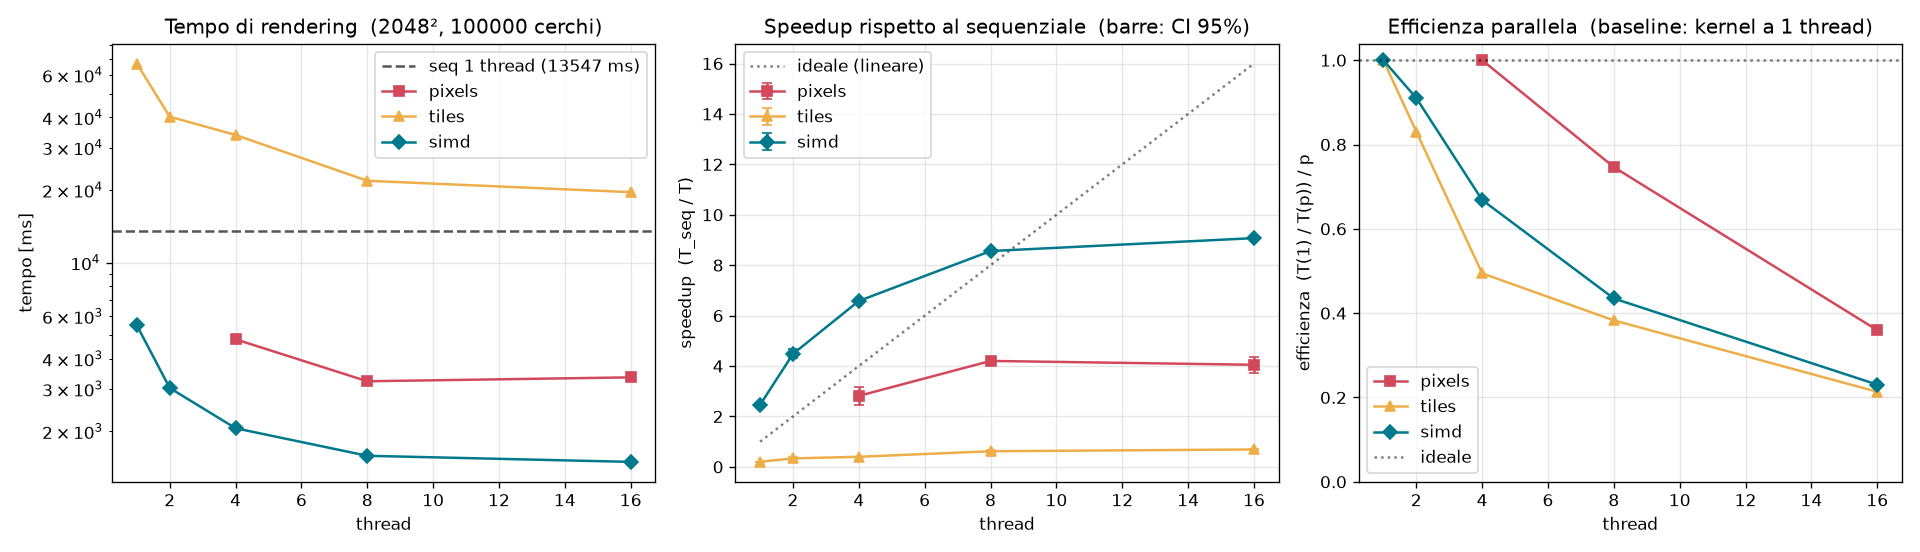
\includegraphics[width=0.95\linewidth]{../figures/bench_scaling.png}
\caption{Strong scaling: rendering time (log scale), speedup vs.\ the
sequential baseline, and parallel efficiency, for all three parallel kernels,
from 1 to 16 (oversubscribed) threads.}
\label{fig:scaling}
\end{figure*}

\begin{table}[h]
\centering
\small
\begin{tabular}{@{}rrrr@{}}
\toprule
\textbf{Threads} & \textbf{Time (ms)} & \textbf{Speedup} & \textbf{Efficiency} \\
\midrule
1  & 5503.5 & 2.46$\times$ & 2.46 \\
2  & 3022.8 & 4.48$\times$ & 2.24 \\
4  & 2058.3 & 6.58$\times$ & 1.65 \\
8  & 1582.2 & 8.56$\times$ & 1.07 \\
16 & 1492.9 & 9.08$\times$ & 0.57 \\
\bottomrule
\end{tabular}
\caption{Strong scaling of the \texttt{simd} kernel on the 100{,}000-circle,
$2048^2$ workload (speedup relative to the 13.55\,s sequential baseline;
efficiency here is $\text{speedup}/p$).}
\label{tab:scaling}
\end{table}

Three effects are visible. First, vectorization alone already gives the
\texttt{simd} kernel a large head start at $p{=}1$ (2.5$\times$ faster than
\texttt{seq} on a single thread), confirming that SIMD and multithreading are
largely independent, additive sources of speedup. Second, all three kernels
scale well up to 4--8 threads, matching the machine's physical core count.
Third, beyond 8 threads (i.e.\ once the thread count exceeds the number of
physical cores, entering oversubscription on the efficiency cores) speedup
flattens for every kernel while efficiency keeps dropping — the extra logical
threads provide diminishing, then negligible, returns. The \texttt{tiles}
kernel (culling, no SIMD) is consistently between \texttt{pixels} and
\texttt{simd}, showing that culling and vectorization are complementary, not
substitutable, optimizations: culling alone (\texttt{tiles}) only reaches
$\sim\!0.7\times$ the sequential kernel's speedup at best, while adding SIMD
on top pushes the maximum speedup to \textbf{9.08$\times$}. On this very
dense workload (100{,}000 large circles) each tile has a long candidate list,
so \texttt{tiles} tests many circles per pixel, whereas \texttt{seq} only
visits the pixels inside each circle's bounding box.

\subsection{Effect of Resolution and Circle Count}

Figures~\ref{fig:resolution}--\ref{fig:circles} sweep image resolution and
circle count independently (at a fixed thread count of 16). Both scale
roughly linearly with problem size for all three kernels tested
(\texttt{seq}, \texttt{tiles}, \texttt{simd}), consistent with the algorithm's
cost being dominated by pixels-inside-bounding-boxes rather than by a
resolution- or count-dependent constant overhead. \texttt{simd} is always
the fastest, 2--5$\times$ faster than \texttt{tiles}, with the gap growing
with problem size. \texttt{tiles} beats \texttt{seq} in most configurations
(at 2048$^2$, \texttt{tiles} is 2.3$\times$ faster than \texttt{seq};
\texttt{simd} is 8.5$\times$ faster), but falls behind it at 8000 circles
(235.8\,ms vs.\ 196.0\,ms): with many circles the per-tile candidate lists
grow long, the same effect seen in the strong-scaling experiment.

\begin{figure}[t]
\centering
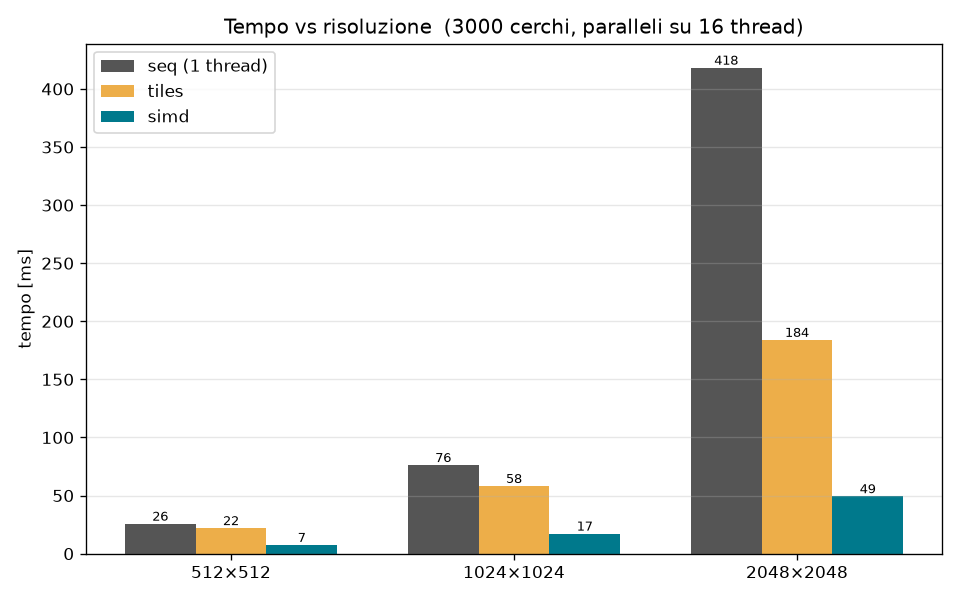
\includegraphics[width=\linewidth]{../figures/bench_resolution.png}
\caption{Rendering time vs.\ image resolution (3000 circles, 16 threads).}
\label{fig:resolution}
\end{figure}

\begin{figure}[t]
\centering
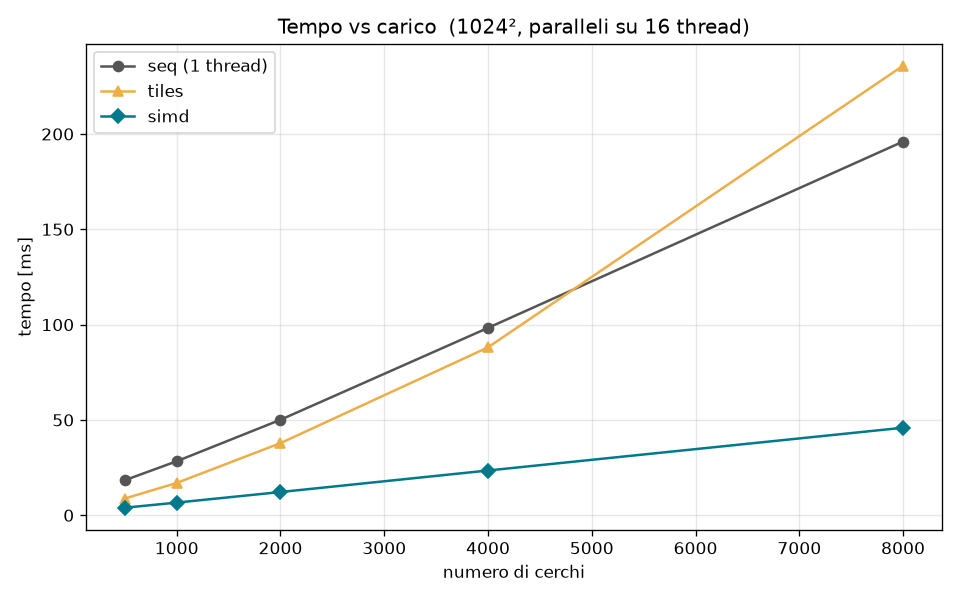
\includegraphics[width=\linewidth]{../figures/bench_circles.png}
\caption{Rendering time vs.\ circle count (1024$^2$ image, 16 threads).}
\label{fig:circles}
\end{figure}

\subsection{Effect of Tile Size}

Figure~\ref{fig:tile} sweeps the tile side length from 16 to 256 pixels
(1024$^2$ image, 4000 circles, 16 threads). \texttt{simd} is fastest at
\textbf{tile~=~32} and \texttt{tiles} at tile~=~16 (with 32 only 10\% slower);
both degrade quickly for larger tiles: bigger tiles mean fewer, coarser parallel work units (worse load
balancing and less L1/L2 residency for the per-tile scratch buffers), while
very small tiles pay a proportionally larger fixed per-tile overhead
(building the candidate list). \texttt{simd} is consistently 3--4.3$\times$
faster than \texttt{tiles} across the whole sweep, and both kernels prefer
small tiles (16--32\,px), so the tile-size sweet spot depends little on
whether the inner loop is vectorized.

\begin{figure}[t]
\centering
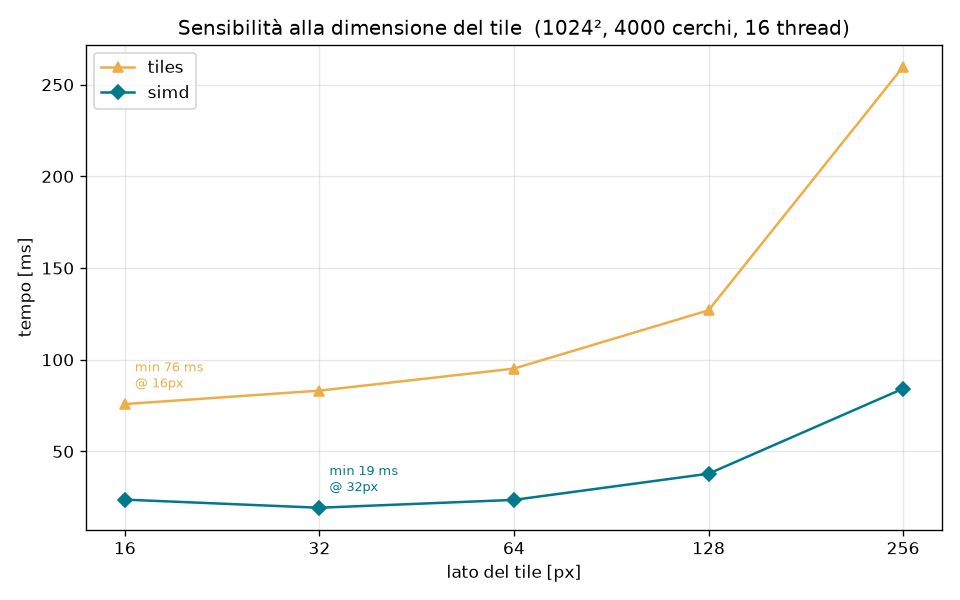
\includegraphics[width=\linewidth]{../figures/bench_tile.png}
\caption{Rendering time vs.\ tile size, for the \texttt{tiles} and
\texttt{simd} kernels.}
\label{fig:tile}
\end{figure}

\subsection{Effect of SIMD (Scalar vs.\ Vectorized)}

To isolate the contribution of vectorization from thread count,
Figure~\ref{fig:simd} compares \texttt{tiles} (scalar inner loop) against
\texttt{simd} (vectorized inner loop) across the same thread sweep (1--16),
at fixed resolution and circle count. At every thread count \texttt{simd} is
faster: \textbf{3.6$\times$} at $p{=}1$ (327.4\,ms vs.\ 91.2\,ms) and still
\textbf{4.0$\times$} at $p{=}16$ (91.1\,ms vs.\ 22.9\,ms). The peak of
5.5$\times$ at $p{=}4$ is partly due to \texttt{tiles} scaling poorly from 2 to
4 threads in this run (184.9\,ms $\to$ 144.1\,ms), rather than to
\texttt{simd} itself. This confirms
that vectorization and multithreading are two genuinely separate levers on
performance, and that neither substitutes for the other.

\begin{figure}[t]
\centering
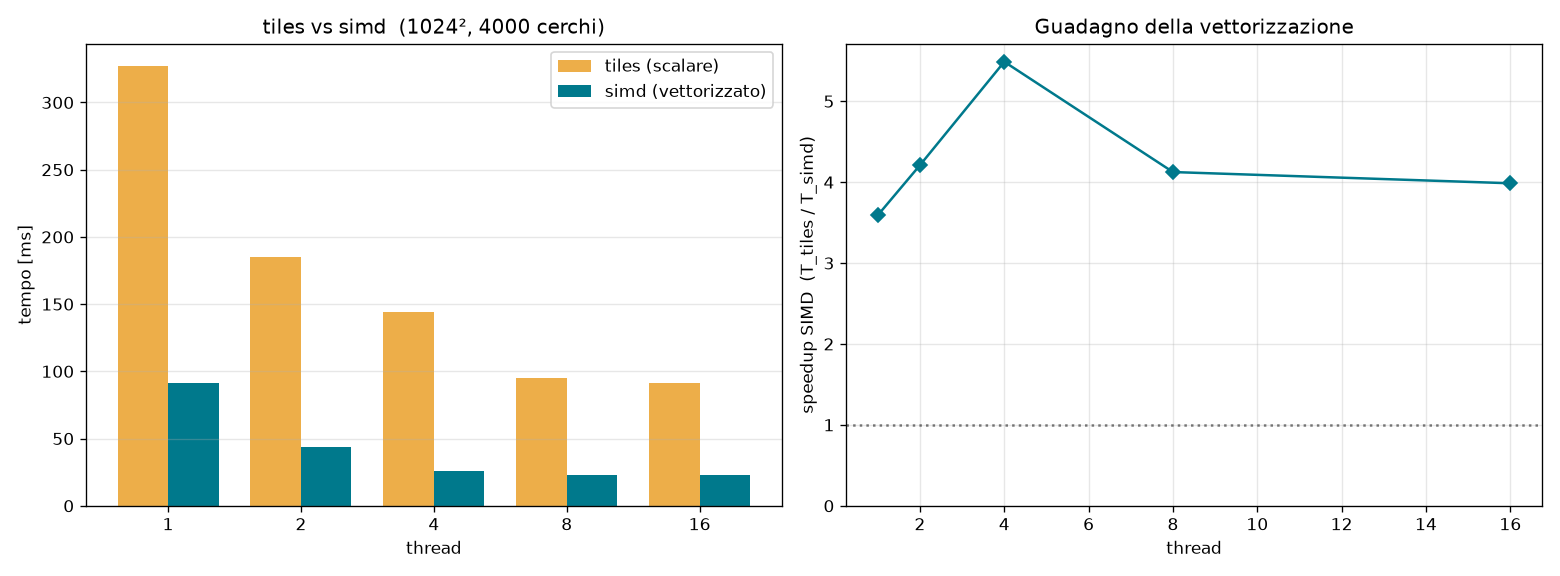
\includegraphics[width=\linewidth]{../figures/bench_simd.png}
\caption{Scalar (\texttt{tiles}) vs.\ vectorized (\texttt{simd}) kernel,
across thread counts 1--16 (1024$^2$ image, 4000 circles).}
\label{fig:simd}
\end{figure}

\subsection{Memory Layout: SoA vs.\ AoS}
\label{sec:memlayout}

Figure~\ref{fig:memlayout} compares the default SoA layout against an
interleaved AoS layout for the otherwise-identical \texttt{tiles} kernel.
The \texttt{tiles} kernel was chosen over \texttt{simd} on purpose: in
\texttt{tiles}, circle attributes are read inside the per-pixel loop (for
every candidate circle at every pixel), so it is the kernel most sensitive to
how circles are laid out in memory. In \texttt{simd}, instead, each circle's
attributes are loaded once per tile, before the vectorized loop, which then
only touches the per-tile R/G/B buffers; since SIMD there works across pixels,
not across circles, the circle layout would have almost no effect. Neither
layout wins \textbf{consistently}: AoS is faster at 512$^2$ (24.5 vs.\
28.9\,ms) and 2048$^2$ (188.5 vs.\ 209.6\,ms), SoA at 1024$^2$ (63.9 vs.\
67.7\,ms). Differences of 6--15\% that change sign from one resolution to the
next point to measurement variability rather than to a real layout effect.
This is expected for this workload: circle attributes are read
once per tile-candidate-test and once per pixel hit, not streamed
sequentially over the whole array in a tight loop, so the unit-stride
advantage of SoA is largely hidden by the small candidate-list sizes and by
cache residency of the per-tile working set — the memory-layout choice
matters far less here than it would for a bulk, streaming numerical kernel.

\begin{figure}[t]
\centering
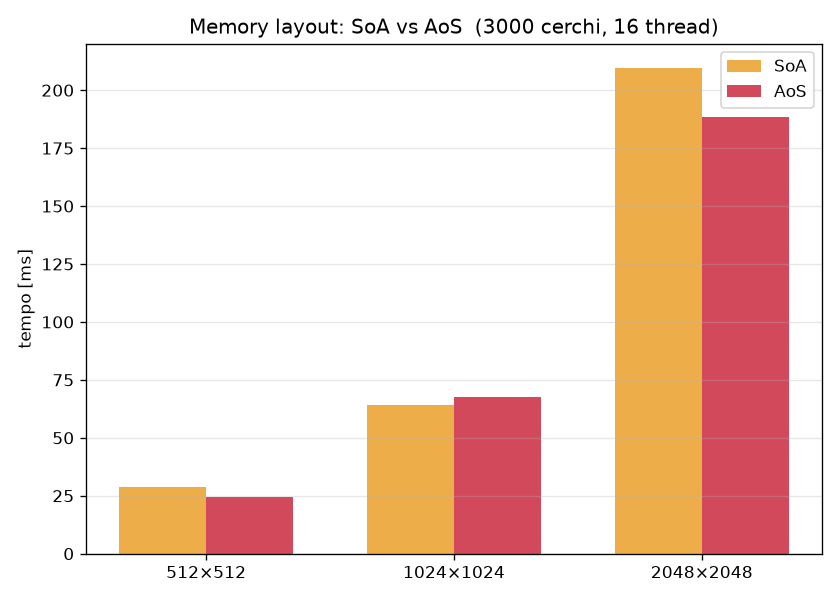
\includegraphics[width=\linewidth]{../figures/bench_memory_layout.png}
\caption{Rendering time, SoA vs.\ AoS circle storage, across resolutions.}
\label{fig:memlayout}
\end{figure}

\subsection{Weak Scaling}

Figure~\ref{fig:weak} keeps work-per-thread constant by growing the circle
count proportionally to the thread count (500 circles per thread). Efficiency
is $\ge\!1.0$ up to 4 threads (i.e.\ within the physical core count, where
larger batches amortize fixed per-call overhead better than the 1-thread
case), then drops to 0.65 at 8 threads and 0.34 at 16. The two drops have
different causes. At 8 threads there is no oversubscription yet (8 threads on
8 cores), but threads 5--8 run on the slower efficiency cores, so the
threads on the performance cores finish early and wait for them. At 16
threads the machine is oversubscribed (16 threads on 8 cores): the extra
threads add no compute and efficiency halves again. Both effects match the
strong scaling result, so they are properties of the machine rather than of
a specific fixed problem size.

\begin{figure}[t]
\centering
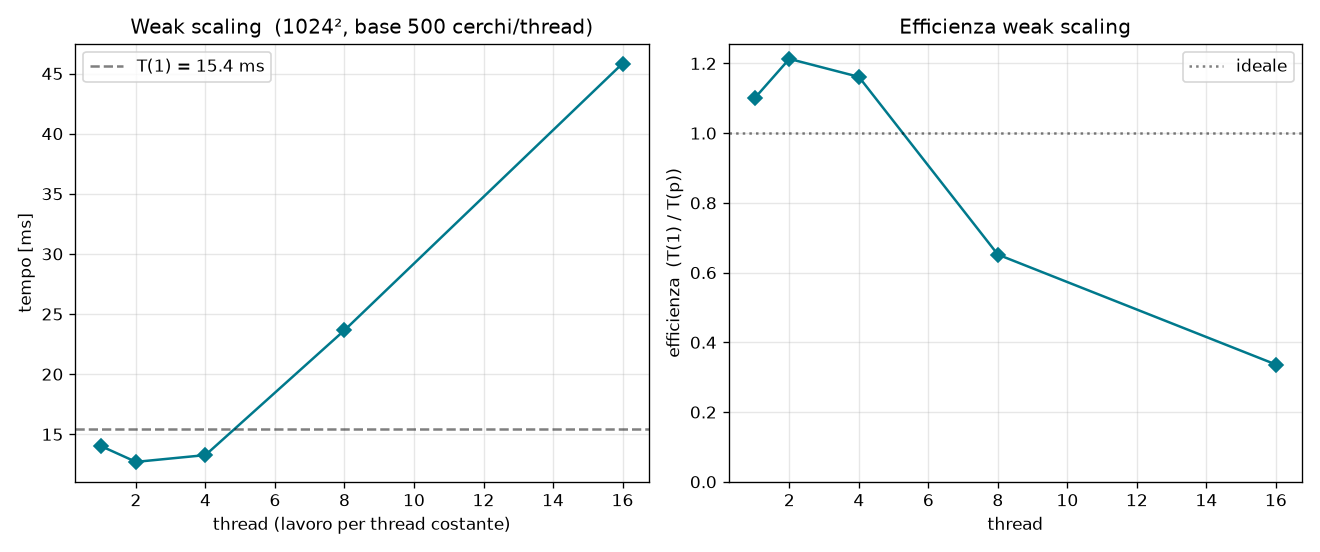
\includegraphics[width=\linewidth]{../figures/bench_weak_scaling.png}
\caption{Weak scaling: circle count grows proportionally with thread count
(500 circles/thread); efficiency relative to the 1-thread baseline.}
\label{fig:weak}
\end{figure}

\subsection{Comparison with Amdahl's and Gustafson's Laws}

Amdahl's law~\cite{amdahl} bounds the speedup on $p$ threads as
$S(p)=1/\bigl(f+(1-f)/p\bigr)$, where $f$ is the fraction of the run that
cannot be parallelized. In the \texttt{simd} wrapper the only serial work is
allocating the image and sorting the circles by $Z$: about 17\,ms out of the
5.5\,s single-thread run on the strong scaling workload, so $f\approx0.003$.
With this $f$, Amdahl predicts $S(8)\approx7.8$ and $S(16)\approx15.3$
relative to \texttt{simd} on one thread. The measured values
(Table~\ref{tab:scaling}) are much lower: $5503.5/1582.2=3.5$ at 8 threads
and $3.7$ at 16. The Karp--Flatt metric
$e=\bigl(1/S(p)-1/p\bigr)/\bigl(1-1/p\bigr)$,
which
estimates the serial fraction from the measured speedup, gives
$e=0.10$, $0.17$, $0.19$ and $0.22$ for $p=2,4,8,16$. It is far above
0.003 and grows with $p$. A growing $e$ indicates that the limit is not
serial code but an overhead that increases with the thread count: the
slower efficiency cores from 5 threads on, thermal throttling under
all-core load, and oversubscription at 16 threads.

Gustafson's law~\cite{robey} describes the weak scaling case, where the
problem grows with $p$: the scaled speedup is $S(p)=p-f\,(p-1)$, so with
$f\approx0.003$ the efficiency should stay close to 1. This matches the
measurements up to 4 threads (efficiency $\ge1.0$,
Fig.~\ref{fig:weak}) but not beyond (0.65 at 8, 0.34 at 16), confirming the
same conclusion: past the performance cores, scaling is limited by the
hardware, not by the serial part of the algorithm.

\subsection{Bottleneck Analysis}

Taken together, the experiments point to two dominant, largely independent
limits on performance:

\begin{itemize}[itemsep=1pt,topsep=2pt]
  \item \textbf{Heterogeneous cores and oversubscription.} Every
    scaling experiment (strong and weak) shows the same qualitative
    behavior: good scaling up to 4 threads (the performance cores), smaller
    gains from 5 to 8 threads, when the slower efficiency cores join in, and
    no further gain beyond 8 threads, where the extra threads only
    oversubscribe the 8 physical cores and add scheduling overhead.
  \item \textbf{Load imbalance from circle-size variance}, which is exactly
    why tile-based \texttt{prange} scheduling and tile-size tuning matter
    more than memory-layout choices for this workload: unlike a dense
    numerical kernel, the bottleneck here is uneven \emph{work} distribution
    across parallel units, not memory bandwidth or cache locality (as
    confirmed by the lack of a consistent SoA/AoS difference).
\end{itemize}

%==================================================================
\section{Conclusions}

This project implemented and systematically benchmarked a CPU-parallel 2D
circle rasterizer, combining coarse-grained multithreading (Numba
\texttt{prange} over image tiles) with fine-grained SIMD vectorization
(a branchless, auto-vectorizable inner loop). The tiled, vectorized kernel
reaches a maximum speedup of \textbf{9.08$\times$} over the sequential
baseline on an 8-core Apple Silicon M2, with vectorization alone contributing
roughly \textbf{4$\times$} independently of thread count. Culling
(tile-based candidate lists) and vectorization proved to be complementary,
additive optimizations rather than substitutes for one another. A dedicated
tile-size sweep identified small tiles (32~px for \texttt{simd}) as the sweet spot for this workload,
and, since tiles are disjoint, the renderer needs no synchronization at all.
Memory layout (SoA vs.\ AoS) had a comparatively minor effect,
consistent with a workload whose bottleneck is irregular per-tile work rather
than memory bandwidth. Both strong and weak scaling confirm that scaling is
good on the 4 performance cores, weaker once the efficiency cores are
involved, and flat under oversubscription beyond 8 threads.

Future work could explore spatial acceleration structures (e.g.\ a
tile-local BVH or grid over circles for very high circle counts), GPU
offload of the tile-based kernel, and adaptive tile sizing driven by local
circle density rather than a single fixed tile size.

%==================================================================
\begin{thebibliography}{9}
\small
\bibitem{slides} Parallel Programming course, Universit\`a degli Studi di
  Firenze, (course slides: assignment
  descriptions, implementation guidelines and technical report structure).
\bibitem{amdahl} G.~M. Amdahl, ``Validity of the single processor approach
  to achieving large scale computing capabilities,''
  \emph{Proc.\ AFIPS Spring Joint Computer Conference}, 1967.
\bibitem{robey} R.~Robey, Y.~Zamora, \emph{Parallel and High Performance
  Computing}, Manning, 2021.
\end{thebibliography}

\vspace{1ex}
\noindent\textbf{Authorship:} I confirm that I am the sole author of this
writeup and the associated code.

\end{document}
